% Poster built with tcolorbox's poster library (grid of named boxes), pdfLaTeX, A0 portrait
\documentclass[a0paper,portrait]{article}
\usepackage[margin=2cm]{geometry}
\usepackage[T1]{fontenc}
\usepackage{newtxtext,newtxmath}
\usepackage[scaled]{helvet}
\usepackage[poster]{tcolorbox}
\usepackage{graphicx,booktabs,tikz,pgfplots}
\pgfplotsset{compat=1.14}
\pgfplotsset{every axis/.append style={tick label style={font=\fontsize{36}{42}\selectfont}, label style={font=\fontsize{40}{48}\selectfont}, legend style={font=\fontsize{36}{42}\selectfont}}}
\pagestyle{empty}
\definecolor{csnavy}{RGB}{31,48,80}
\definecolor{csteal}{RGB}{42,157,176}
\definecolor{csbord}{RGB}{96,0,48}
\definecolor{csgrey}{RGB}{150,150,150}
\definecolor{paleteal}{RGB}{230,244,247}
\newcommand{\placeholder}[2]{\begin{center}\fbox{\begin{minipage}[c][#1][c]{0.92\linewidth}\centering\fontsize{40}{48}\selectfont #2\end{minipage}}\end{center}}

\begin{document}
\fontsize{40}{48}\selectfont
\begin{tcbposter}[
  poster = {width=\linewidth, height=\textheight, columns=3, rows=7, spacing=8mm, showframe=false},
  boxes  = {enhanced standard, colback=white, colframe=csnavy, arc=2mm, boxrule=1pt,
    colbacktitle=csnavy, coltitle=white, fonttitle=\sffamily\bfseries\fontsize{46}{54}\selectfont,
    left=6mm, right=6mm, top=4mm, bottom=4mm, fontupper=\fontsize{40}{48}\selectfont}
]

\posterbox[colback=csnavy,colframe=csnavy,halign=center,valign=center,
  fontupper=\sffamily\color{white}]{name=title,column=1,span=3,row=1,rowspan=1}{
  {\bfseries\fontsize{76}{84}\selectfont Can ten qubits finish your sentence?}\\[3mm]
  {\fontsize{36}{42}\selectfont Not better than a small classical network: three quantum language models tested against fair controls}\\[3mm]
  {\fontsize{30}{36}\selectfont Ethan Bandasack, Malo Leroy, Thierry Zhang \textperiodcentered{} Supervisor: Zeno Toffano \textperiodcentered{} CentraleSupélec, Université Paris-Saclay, L2S}\\[3mm]
  {\fontsize{30}{36}\selectfont AI and OneHealth workshop, 20 November 2026}
}

\posterbox[adjusted title=Why quantum semantics?]{name=why,column=1,span=1,row=2,rowspan=2}{
  Quantum-like semantics writes word meanings as vectors and relations between them as operators. Contraries, contradictions and inclusions of the semiotic square become Pauli operators (Galofaro et al., 2018; Dubois and Toffano, 2026). A cosine similarity confuses antonyms, which often share contexts; this vocabulary separates them.
  \placeholder{12cm}{Figure: semiotic square with $\sigma_z$ (contraries), $\sigma_x$ (contradictions), $\sigma_y$ (inclusion)}
}

\posterbox[adjusted title={Three models, one rule}]{name=models,column=2,span=1,row=2,rowspan=2}{
  Every classical control gets the same inputs, targets and training budget.
  \begin{center}\fontsize{30}{36}\selectfont
  \begin{tabular}{lll}
  \toprule
  Model & Qubits & Readout \\
  \midrule
  QCSE, reimplemented & 14 & bit-wise $Z$ marginals \\
  Hybrid circuit & 8 & classical head \\
  Hamiltonian predictor & 10 & Born rule, no head \\
  \bottomrule
  \end{tabular}
  \end{center}
}

\posterbox[adjusted title={Take-home},colback=paleteal,colframe=csteal,colbacktitle=csteal]{name=takehome,column=3,span=1,row=2,rowspan=2}{
  \begin{itemize}
  \item No quantum advantage: every quantum or hybrid model was matched or beaten by a classical model with the same information.
  \item Check the metric first: a constant guess scores $96.5\%$ on the published criterion.
  \item Always run the identity control.
  \end{itemize}
}

\posterbox[adjusted title={1 \quad A constant guess beats the published metric}]{name=res1,column=1,span=1,row=4,rowspan=3}{
  The published score counts a word as right when half of its bits match. A constant prior scores $96.5\%$; QCSE scores $56.1\%$ and recovers no word exactly.
  \begin{center}
  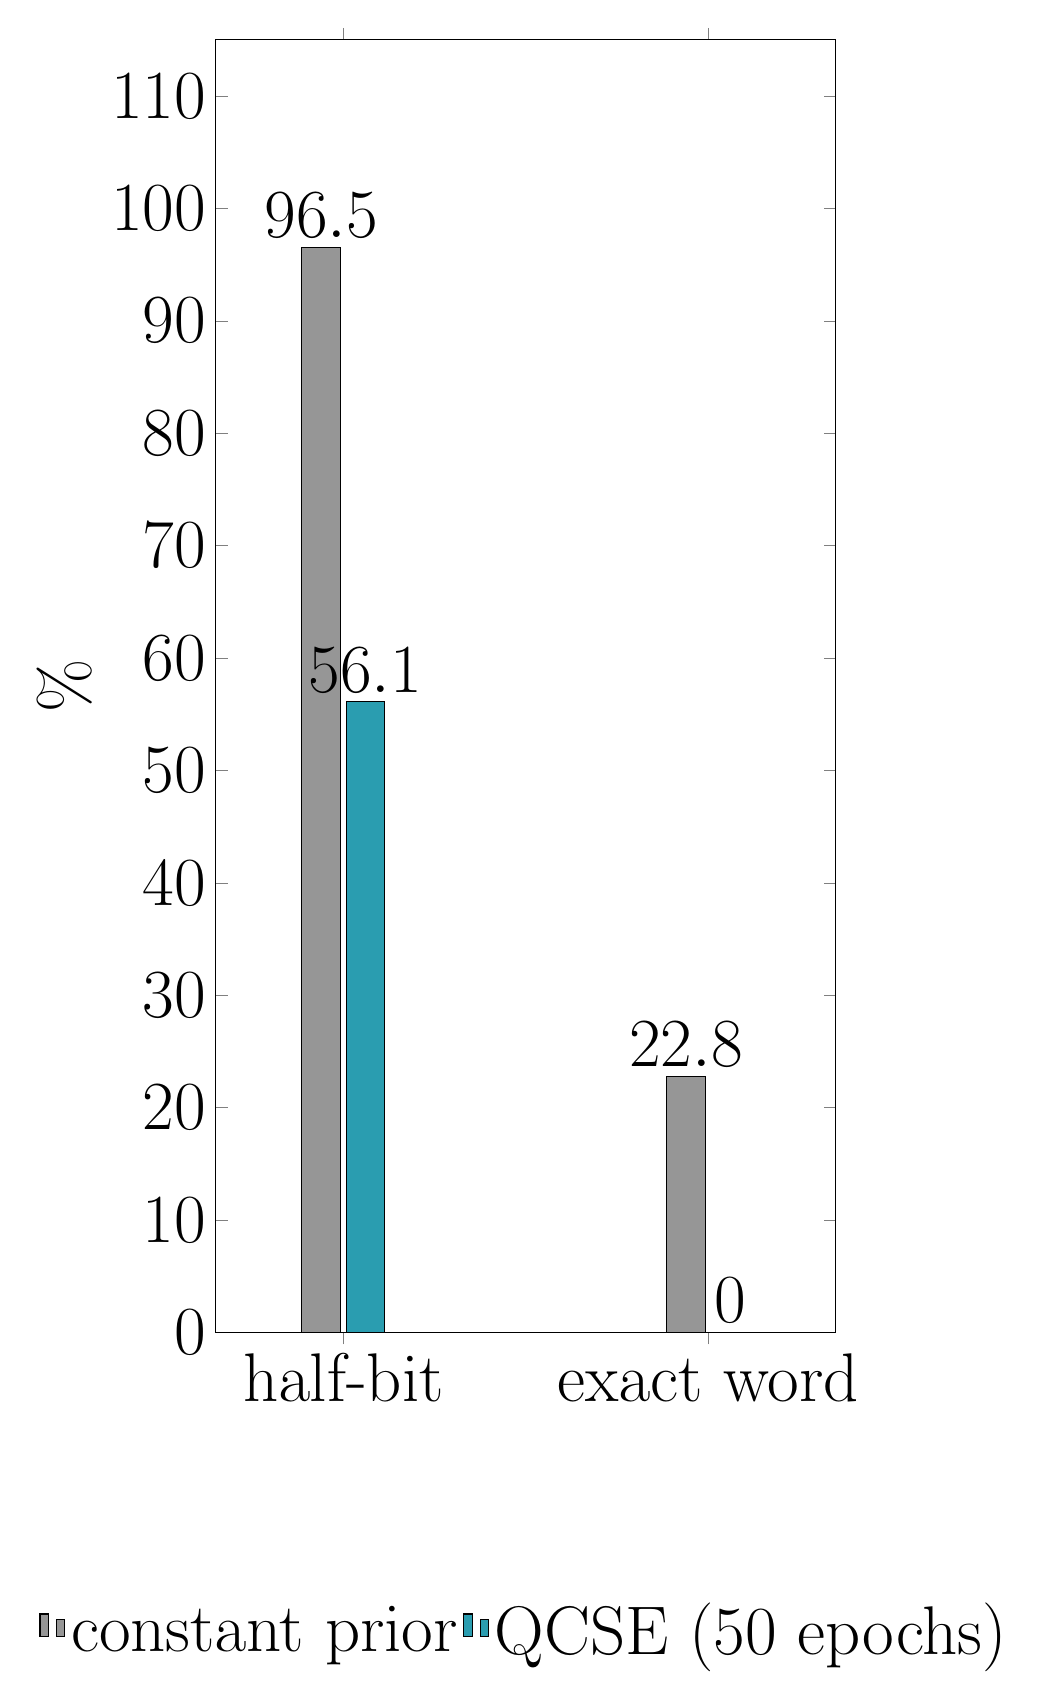
\begin{tikzpicture}
  \begin{axis}[ybar, bar width=14pt, width=0.78\linewidth, height=18cm, ymin=0, ymax=115, ylabel={\%},
    symbolic x coords={half-bit, exact word}, xtick=data, enlarge x limits=0.35,
    legend style={at={(0.5,-0.2)},anchor=north,legend columns=2,draw=none,font=\fontsize{36}{42}\selectfont},
    nodes near coords, nodes near coords style={font=\fontsize{36}{42}\selectfont}]
  \addplot[fill=csgrey] coordinates {(half-bit,96.5) (exact word,22.8)};
  \addplot[fill=csteal] coordinates {(half-bit,56.1) (exact word,0.0)};
  \legend{constant prior, QCSE (50 epochs)}
  \end{axis}
  \end{tikzpicture}
  \end{center}
}

\posterbox[adjusted title={2 \quad Remove the circuit, and nothing changes}]{name=res2,column=2,span=1,row=4,rowspan=3}{
  Bidirectional top-1 accuracy: $50.4\%$ with a trained circuit, $50.0\%$ with the identity circuit, $54.9\%$ with an MLP.
  \begin{center}
  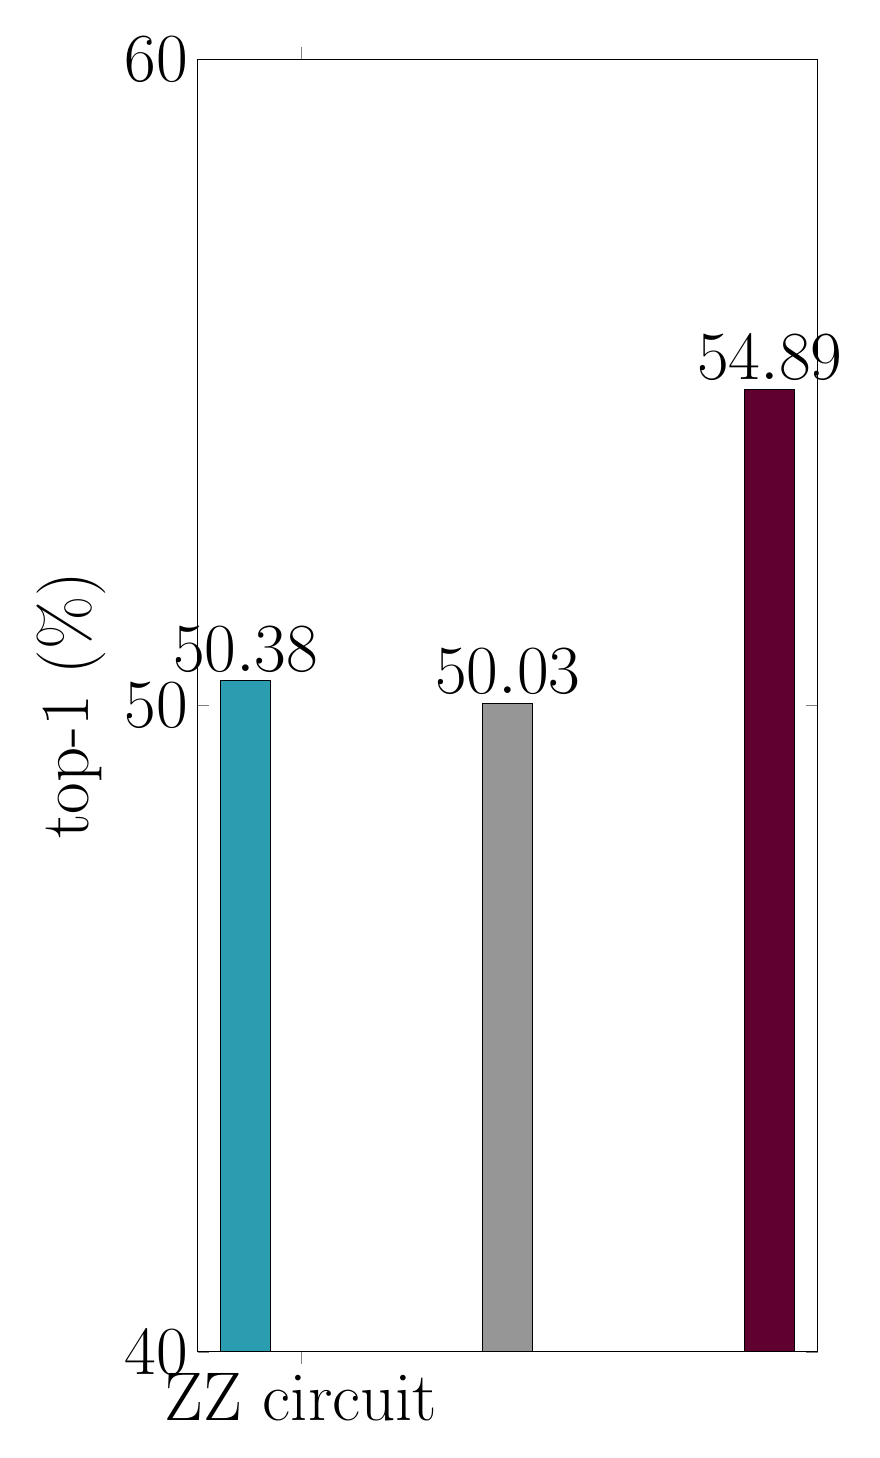
\begin{tikzpicture}
  \begin{axis}[ybar, bar width=18pt, width=0.78\linewidth, height=18cm, ymin=40, ymax=60, ytick={40,50,60}, ylabel={top-1 (\%)},
    symbolic x coords={ZZ circuit, identity, MLP-32}, xtick=data, enlarge x limits=0.25,
    nodes near coords, nodes near coords style={font=\fontsize{36}{42}\selectfont}]
  \addplot[fill=csteal] coordinates {(ZZ circuit,50.38)};
  \addplot[fill=csgrey] coordinates {(identity,50.03)};
  \addplot[fill=csbord] coordinates {(MLP-32,54.89)};
  \end{axis}
  \end{tikzpicture}
  \end{center}
}

\posterbox[adjusted title={3 \quad It learns, but the MLP stays ahead}]{name=res3,column=3,span=1,row=4,rowspan=3}{
  On WikiText-2 subwords the quantum NLL falls from $4.28$ to $2.47$ nats; the MLP reaches $2.22$. Coherence helps against a dephased copy, not against a classical network.
  \begin{center}
  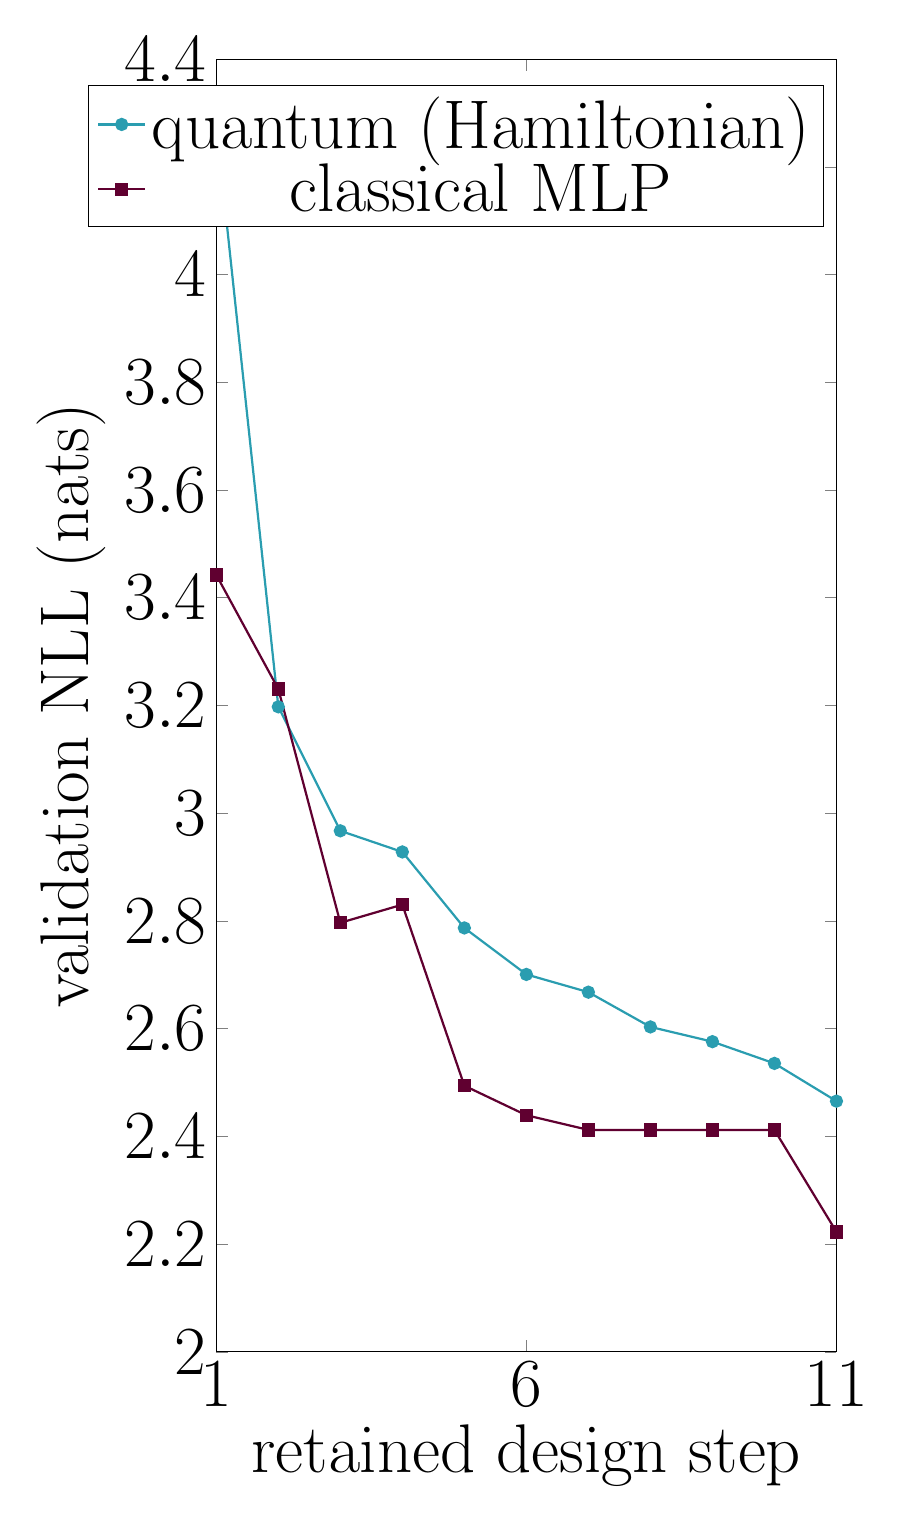
\begin{tikzpicture}
  \begin{axis}[width=0.78\linewidth, height=18cm, ylabel={validation NLL (nats)}, xlabel={retained design step},
    xmin=1, xmax=11, xtick={1,6,11}, ymin=2, ymax=4.4, legend style={at={(0.98,0.98)},anchor=north east,font=\fontsize{36}{42}\selectfont}]
  \addplot[thick, csteal, mark=*] coordinates {
    (1,4.2773) (2,3.1975) (3,2.9673) (4,2.9281) (5,2.7870) (6,2.7007)
    (7,2.66776) (8,2.60325) (9,2.57588) (10,2.53554) (11,2.46546)};
  \addlegendentry{quantum (Hamiltonian)}
  \addplot[thick, csbord, mark=square*] coordinates {
    (1,3.4424) (2,3.2306) (3,2.7966) (4,2.8303) (5,2.4941) (6,2.4393)
    (7,2.41207) (8,2.41207) (9,2.41207) (10,2.41207) (11,2.22277)};
  \addlegendentry{classical MLP}
  \end{axis}
  \end{tikzpicture}
  \end{center}
}

\posterbox[adjusted title=What it means]{name=meaning,column=1,span=1,row=7,rowspan=1}{
  \begin{itemize}
  \item Most gains came from classical ingredients: learned embeddings, count priors, context pooling.
  \item Limits: noiseless simulation, two or three seeds, WikiText test split left unscored.
  \item Next: test the semiotic square directly on a relation-classification task.
  \end{itemize}
}

\posterbox[adjusted title={References},colback=white]{name=refs,column=2,span=1,row=7,rowspan=1}{
  \fontsize{36}{42}\selectfont
  \begin{itemize}
  \item Bengio, Ducharme, Vincent, Jauvin (2003). A neural probabilistic language model. JMLR.
  \item Coecke, Sadrzadeh, Clark (2010). Mathematical foundations for a compositional distributional model of meaning.
  \item Dubois, Toffano (2026). On quantum relations. Entropy.
  \item Galofaro, Toffano, Doan (2018). A quantum-based semiotic model for textual semantics. Kybernetes.
  \item Varmantchaonala et al. (2026). QCSE. arXiv:2509.05729.
  \end{itemize}
}

\posterbox[adjusted title={Credits and code},colback=white]{name=credits,column=3,span=1,row=7,rowspan=1}{
  Laboratoire des Signaux et Systèmes (L2S), CentraleSupélec, Université Paris-Saclay. Supervisor: Zeno Toffano.
  \vspace{4mm}\\
  
\includegraphics[height=4cm]{CS}\hfill
\includegraphics[height=3.4cm]{L2S_logo}
}

\end{tcbposter}
\end{document}
